%===================================================================================
\subsection{CU22 Visualizar datos de la tarea}
{
\justify
\color{blue}{\textbf{Objetivo}}
}

%------------------------------------------------------------------
\justify
Permite al Lider de proyecto visualizar los datos que componen a la tarea.
%------------------------------------------------------------------
{
\justify
\color{blue}{\textbf{Diseño}}
}
%-------------------------------------------------------------------------------
\justify
En la figura \ref{fig:IU23} se muestra la pantalla, en donde permite al Lider de proyecto visualizar los datos que componen a la tarea.

\begin{figure}[htb]
\centering
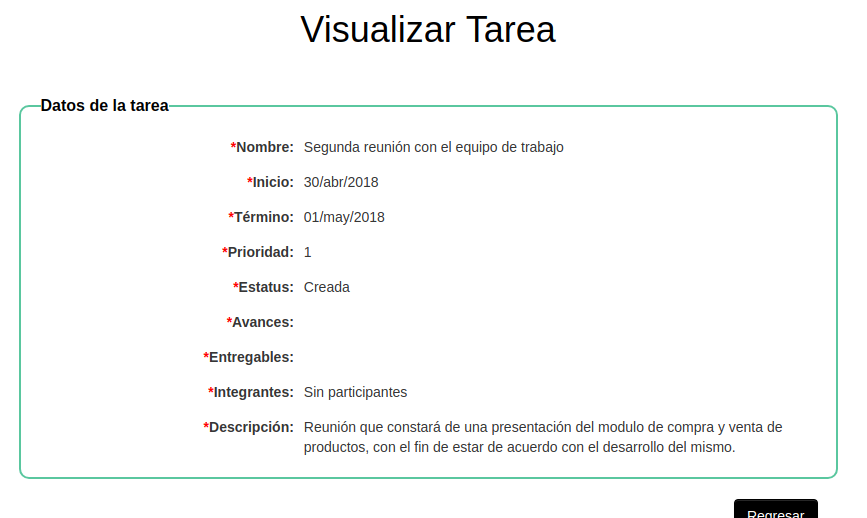
\includegraphics[width=0.8\textwidth]{./images/cu23-visualizar-datos-tarea.png}
\caption{Relacionar tareas.} \label{fig:IU23}
\end{figure}